% !TEX encoding = UTF-8 Unicode
\documentclass[sigconf]{acmart}

\usepackage{booktabs} % For formal tables
\usepackage[utf8]{inputenc}
\usepackage{comment}

% Copyright
%\setcopyright{none}
%\setcopyright{acmcopyright}
%\setcopyright{acmlicensed}
%\setcopyright{rightsretained}.
%\setcopyright{usgov}
%\setcopyright{usgovmixed}
%\setcopyright{cagov}
%\setcopyright{cagovmixed}

% DOI
%\acmDOI{10.1145/3266237.3266249}

% ISBN
%\acmISBN{978-1-4503-6503-1/18/09}

%Conference
%\acmConference[SBES'2018]{SBES Conference}{2018}
%{S\~ao Carlos, S\~ao Paulo, Brazil}
%\acmYear{2018}
%\copyrightyear{2018}

%\acmArticle{4}
%\acmPrice{15.00}

\copyrightyear{2018} 
\acmYear{2018} 
\setcopyright{acmcopyright}
\acmConference[SBES 2018]{XXXII BRAZILIAN SYMPOSIUM ON SOFTWARE ENGINEERING}{September 17--21, 2018}{Sao Carlos, Brazil}
\acmBooktitle{XXXII BRAZILIAN SYMPOSIUM ON SOFTWARE ENGINEERING (SBES 2018), September 17--21, 2018, Sao Carlos, Brazil}
\acmPrice{15.00}
\acmDOI{10.1145/3266237.3266249}
\acmISBN{978-1-4503-6503-1/18/09}

% These commands are optional
%\acmBooktitle{Transactions of the ACM Woodstock conference}
%\editor{Jennifer B. Sartor}
%\editor{Theo D'Hondt}
%\editor{Wolfgang De Meuter}


\begin{document}
\title{FLOSS in Software Engineering Education}
\subtitle{An Update of a Systematic Mapping Study}

\author{Moara Sousa Brito}
\affiliation{%
  \institution{Federal University of Bahia}
  \city{Salvador}
  \state{Brazil}
}
\email{moara.brito@ufba.br}

\author{Fernanda Gomes Silva}
\affiliation{%
  \institution{Federal University of  Bahia}
  \city{Salvador}
  \state{Brazil}
}
\email{fernanda_gomes@unit.br}

\author{Christina von Flach G. Chavez} 
\affiliation{%
  \institution{Federal University of  Bahia}
  \city{Salvador}
  \state{Brazil}
}
\email{flach@ufba.br}

\author{Debora C. Nascimento} 
\affiliation{%
  \institution{Federal University of Sergipe}
  \city{Aracaju}
  \state{Brazil}
}
\email{dmcnascimento@ufs.br}

\author{Roberto A. Bittencourt} 
\affiliation{%
  \institution{State University of Feira de Santana}
  \city{Feira de Santana}
  \state{Brazil}
}
\email{roberto@uefs.br}


% The default list of authors is too long for headers.
\renewcommand{\shortauthors}{M. Brito et al.}

\begin{abstract}
% abstract

\textbf{Context:}
Free/Libre/Open Source Software (FLOSS) projects
have been used in Software Engineering Education (SEE)
to address the need for more realistic settings
that reduce the gap between
software engineering (SE) courses and industry needs.
A systematic mapping study (SMS) performed in 2013
structured the research area on the use of FLOSS projects in SEE.
%
\textbf{Objective:} 
Update the 2013 SMS with studies published in the last five years,
classifying and summarizing them
to discuss trends and identify research gaps
in the context of the use of FLOSS projects in SEE.
%
\textbf{Method:} 
We retrieved and analyzed a set of 4132 papers 
published from 2013 to 2017,
from which 33 papers were selected and classified.
%according to the scheme proposed in the original SMS.
We analyzed the new results and compared them
with those from the previous SMS
to confirm or discover trends.
%
\textbf{Results:} 
The updated mapping summarizes
the studies published in the last five years,
most of them in conferences.
Our analysis confirmed trends previously observed for three facets
(SE area, curriculum choice and assessment type) and discovered new trends for other facets.
%
\textbf{Conclusion:}
Studies report the use of FLOSS projects
in regular, comprehensive SE courses.
The prevalence of experience reports
over solution proposals %as a research type
in the last five years may indicate that
researchers are more concerned with the use and evaluation
of existing proposals, although there are still opportunities
for more empirical work based on 
sound educational research methods.


\end{abstract}

%
% The code below should be generated by the tool at
% http://dl.acm.org/ccs.cfm
% Please copy and paste the code instead of the example below.
%
\begin{CCSXML}
<ccs2012>
<concept>
<concept_id>10003456.10003457.10003527.10003531.10003751</concept_id>
<concept_desc>Social and professional topics~Software engineering education</concept_desc>
<concept_significance>500</concept_significance>
</concept>
<concept>
<concept_id>10011007</concept_id>
<concept_desc>Software and its engineering</concept_desc>
<concept_significance>500</concept_significance>
</concept>
<concept>
<concept_id>10011007.10011074.10011134.10003559</concept_id>
<concept_desc>Software and its engineering~Open source model</concept_desc>
<concept_significance>500</concept_significance>
</concept>
<concept>
<concept_id>10002944.10011122.10002945</concept_id>
<concept_desc>General and reference~Surveys and overviews</concept_desc>
<concept_significance>300</concept_significance>
</concept>
</ccs2012>
\end{CCSXML}

\ccsdesc[500]{Social and professional topics~Software engineering education}
\ccsdesc[500]{Software and its engineering}
\ccsdesc[500]{Software and its engineering~Open source model}
\ccsdesc[300]{General and reference~Surveys and overviews}

\keywords{Free software, open source software, FLOSS development model, systematic literature reviews.}

\maketitle

\section{Introduction} \label{sec:introduction}
% Introduction

%Context
Free/Libre/Open Source Software (FLOSS) projects
have been used in Software Engineering Education (SEE)
to address the need for more realistic settings
that could reduce the gap between
software engineering courses and industry needs.
%Several aspects of open source development have pedagogical benefit in a computer science or software engineering program. 
The study of FLOSS projects exposes students to 
large projects, best practices and professional tools 
for version control, build automation, and project management, 
while allowing them to experience the collaborative, social dynamics of team working on these large projects~\cite{Horstmann:2009}.

The most recent systematic mapping study (SMS)  \cite{Petersen,Budgen}
that investigated the use of FLOSS projects in SEE,
structured the research area according to nine facets and
provided an overview of initiatives and research gaps
based on work published prior to 2013 \cite{2015:CSE:nascimento}.
% Main Results 
This SMS identified active research communities, long-term projects and venues for publication, and provided an overview of objectives, contributions and methods applied in 72 studies over 14 years (1998-2012). 
This work provided a baseline for the scholarship on SEE with FLOSS, describing previous work in terms of research/scholarship type, software engineering area, curriculum choice, FLOSS choice, control level, goals and assessment. Results from selected papers showed a gap in the use of sound research methods, a lack of more active learning approaches as well a lack of educational theory foundations. Most selected papers were published in conferences, describing either solution proposals or experience reports on comprehensive software engineering courses based on the traditional project method approach. Interestingly, this paper showed both the community interest of using FLOSS in SEE and the need to improve scholarship to turn this area into a mature field of research.

\begin{figure*}[tb]
\centering
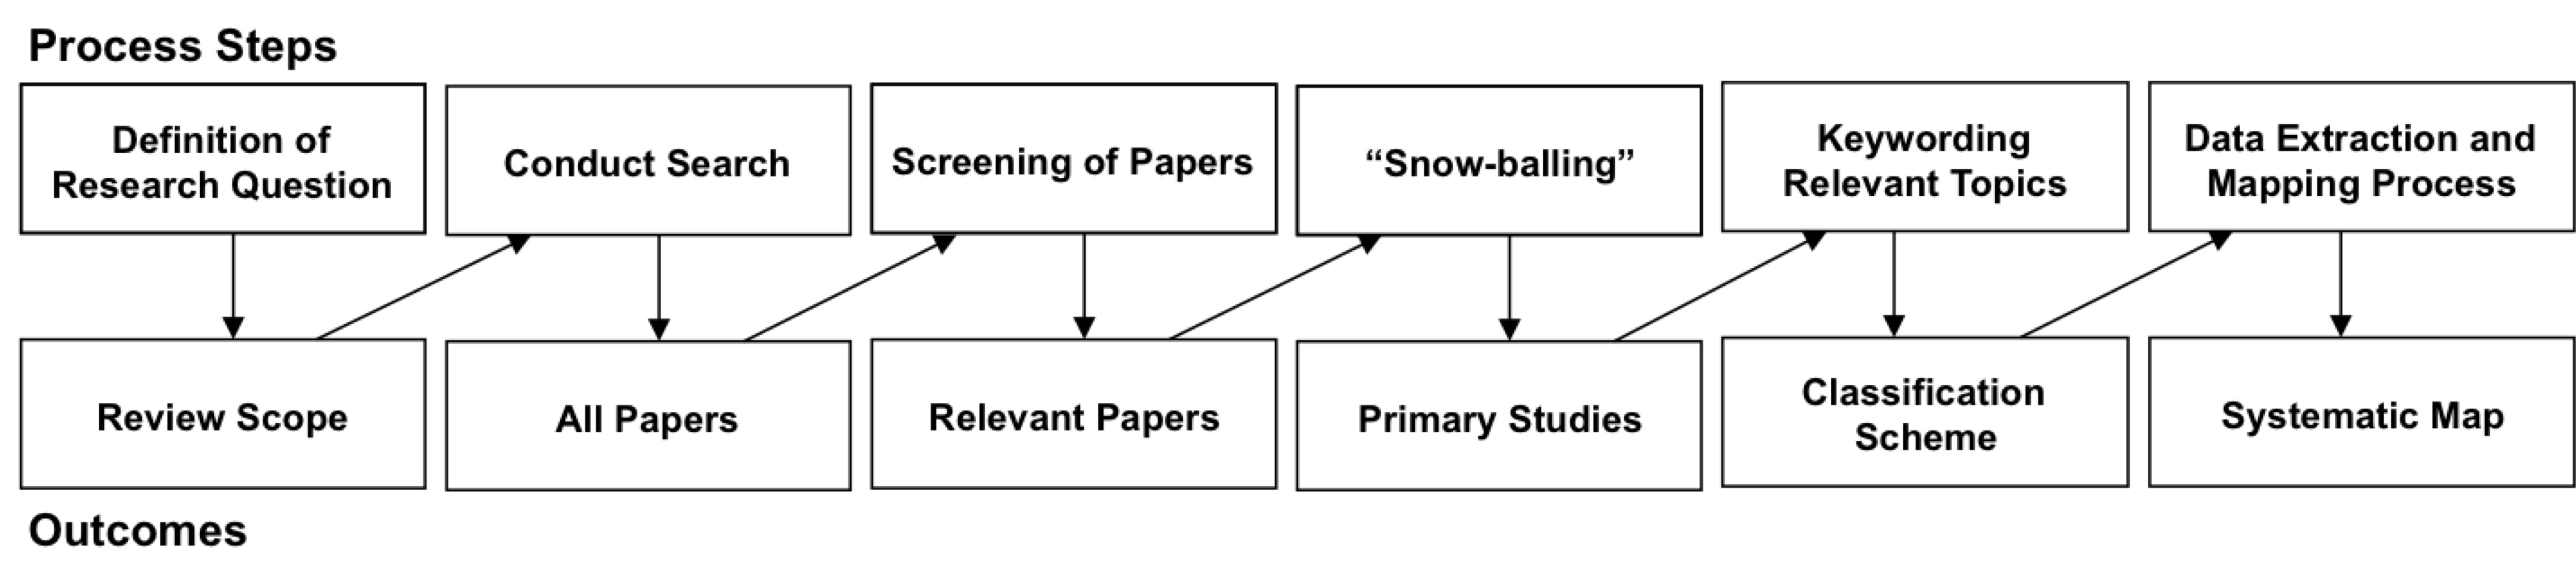
\includegraphics[width=1\linewidth]{fig/update-process.jpg}
\caption{The update process, adapted from \cite{Petersen,2015:CSE:nascimento}.}
\label{fig_smsProcess3}
\end{figure*}
 
The SIGCSE 2016 Panel on ``How to Use Open Source Software in Education'' capitalized on the uses of FLOSS in education, 
pointing out to barriers to its use in educational settings and 
the need for a debate to better take advantage of the collaborative ways to solve hard problems that open source communities and their ecosystems bring \cite{Bishop:2016}.

% The need for an update. WHY? Justify.
Therefore, an updated SMS represents an important 
asset in a new research field that brings together 
FLOSS and SEE, where the number of studies and the maturity of empirical methods used are increasing.

% Talk a little bit about the need for an update.
% This work:
In this work, we present an update of the SMS on 
the use of FLOSS projects in 
SEE~\cite{2015:CSE:nascimento}.
% Talk a little bit more about the update.
We retrieved and analyzed papers published from 2013 to 2017,
and classified them according to the facets used in the original SMS.
% How many facets are presented here and WHY?
We analyzed the new results and compared them
with those from the previous SMS 
to confirm trends and discover new ones.

Our main findings point out both a confirmation of previous research trends as well as some changes that slowly move the field into a more mature research topic. Confirmed trends are: 
(1)~the use of FLOSS to learn comprehensively on software engineering; (2)~curriculum choice particularly focused on regular courses; and 
(3)~assessment mainly based on reports and software artifacts. 
On the other hand, new trends point to: 
(4)~increased use of experience reports and a reduction in solution proposals; 
(5)~growing interest of using FLOSS in software maintenance and evolution; 
(6)~increased use of approaches where instructors have no control, and students interact with the FLOSS community in real tasks; 
(7)~less use of predefined FLOSS projects and more free project choice by students; 
(8)~balance between goals of learning FLOSS and learning SE concepts; and (9)~the use of automated test suites as a relevant assessment type.    

%\textit{Paper Structure.}
The rest of the paper is organized as follows.
Section~\ref{sec:sms:process} presents information about process steps 
performed and outcomes generated in the context of the SMS update.
Section~\ref{sec:updated:sms} presents the results of the updated mapping and compares them with results from the 2013 SMS.
%Section~\ref{sec:trends} discusses ... and trends.
Section~\ref{sec:conclusion} presents contributions and discloses opportunities for future research.




\section{The SMS Update Process} \label{sec:sms:process}
% \section{The Systematic Mapping Study Update Process} \label{sec:sms:process}
% The update process

Figure~\ref{fig_smsProcess3} presents the process 
that guided our update to the SMS conducted by~\citet{2015:CSE:nascimento}.
%Steps marked with \verb1*1 were reused from the previous SMS. 
%Their related outcomes (e.g., review scope and classification scheme),
%were the same as defined in~\cite{2015:CSE:nascimento}.
%
We used the StArt (State of the Art through Systematic Review) tool\footnote{http://lapes.dc.ufscar.br/tools/start\_tool}
and spreadsheets to manage the
data generated during the update process.

%\paragraph{Research Questions}  
The three research questions defined by
~\citet{2015:CSE:nascimento} were also reused in this update:
both the main question and the two secondary questions.
In this paper, we focus on the main research question:

\begin{description}
\item [RQ1.] How are Open Source Projects used in Software Engineering Education? 
\end{description}

%\begin{description}
%\item [RQ2.] Which of the initiatives combine open source projects with active learning in software engineering courses?
%\end{description}
%\begin{description}
%\item [RQ3.] How is student learning assessed in the reviewed initiatives?
%\end{description}

The review scope included the same search strings 
and inclusion/exclusion criteria defined by
~\citeauthor{2015:CSE:nascimento} 
for paper searching and screening.
Detailed information on the SMS protocol
can be found at the original SMS website\footnote{https://sites.google.com/site/dmcnascimento/mapping} 
and detailed information on the updated SMS protocol is available as supplementary material\footnote{https://github.com/Moara/mapping/blob/master/Disponibilizar/Protocolo.pdf}.
% original SMS \cite{2015:CSE:nascimento}.

\subsection{Search}
We conducted the search from March 22 to April 28, 2018. 
The search strategy included 
the same scientific electronic databases
used by~\citet{2015:CSE:nascimento}:
Engineering Village\footnote{http://www.engineeringvillage.com},
IEEE Xplore\footnote{http://ieeexplore.ieee.org}, 
ACM\footnote{http://portal.acm.org}, 
Scopus\footnote{http://www.info.sciverse.com/scopus}, 
Springer\footnote{http://www.springer.com} and 
Science Direct\footnote{http://www.elsevier.com}.
We retrieved 18,056 papers, 
from which 13,924 were duplicates 
(various studies were indexed by more than one digital library), 
leading to 4,132 papers selected for screening.

\subsection{Screening}
Four inclusion criteria (IC) and 20 exclusion criteria (EC) 
defined by~\citet{2015:CSE:nascimento} were reused. 
For instance: 
(IC.1)~Studies that address the use of FLOSS projects to learn/teach Software Engineering should be included, regardless of their application in either SE programs or in other programs;
%(e.g. Computer Science, Computer Engineering, Information Systems, Information Technology or Informatics);
(EC.1)~Documents written in languages other than English should be excluded; (EC.2)~Documents whose full text is not available should be excluded; and (EC.3)~Studies whose main content is not related to learning or teaching Software Engineering should be excluded.

We applied two filters during screening.
First, the two first authors individually examined title and abstract
of each primary study, and marked
each study as either included or excluded. 
A third reviewer compared the results,  
analyzed conflicts and took the final decision. 
In this first step, 39 studies were included.

Then, the two first authors reexamined 
the remaining studies, 
skimming through introduction and conclusion. 
A third reviewer compared their results, 
and again, took the final decision, 
resulting in 33 primary studies selected 
for classification.

%MMMM studies. 
%Finally,  we followed a ``snow-balling'' procedure~\cite{Budgen} that supported us in the identification of other PPPP relevant studies.
%Todos os artigos foram baseadas na string de busca, não fizemos snow-balling.
%A total of 33 primary studies were selected for classification.

\begin{table*}[tb]
%\begin{table}
	\centering
	\caption {Defined Facets~\cite{2015:CSE:nascimento}}  
		{\begin{tabular}{c|l|p{5in}} 
			 & \bf Facet & \bf Description \\
			\hline
			\bf 1 	& \small \bf Software Engineering Area 
            		& The SE topic(s) addressed in the study 
(software engineering in general, requirements, models and methods, design and architecture, quality, testing, evolution and maintenance, development and construction, process, management and configuration management), based on the SWEBOK \citeyearpar{swebok}. \\
			\bf 2 & \small \bf Research Type & The research approach used in the paper 
            	(experience report, case study, action research, experiment/quasi-experiment, survey, opinion paper, solution proposal, philosophical paper
            -- adapted from \citet{Petersen}). \\
%Table~\ref{tab:researchTypeStudies} provides a description of each category,  \\
%			\bf 3 & Learning Approach & The pedagogical approach that was applied together with OSP in SE courses. Table~\ref{tab:activeLearning} presents a description of each category. \\
%			\bf 4 & Assessment Perspective & The perspective from which student learning is evaluated -- see Table~\ref{tab:assessmentPerspective}. \\
			\bf 3 & \small \bf Learning Approach & The pedagogical approach 
            that was applied together with FLOSS projects in SE courses 
            -- not presented in this paper. \\
			\bf 4 & \small \bf Assessment Perspective & The perspective from which
            student learning is evaluated -- not presented in this paper. \\
			\bf 5 & \small \bf Assessment Type & The instrument used to assess student
            learning -- see Table~\ref{tab:assessmentType}. \\
			\bf 6 & \small \bf Approach Goal & Which goal in introducing FLOSS projects
            in SE courses was prevalent (either learning SE principles/concepts 
            or learning to develop FLOSS). \\
			\bf 7 & \small \bf Curriculum Choice & How the content was embodied in
            curriculum -- see Table~\ref{tab:curriculumApproach}. \\
			\bf 8 & \small \bf Control Level & How much control faculty/staff 
            had on the FLOSS project -- see Table~\ref{tab:controlLevel}. \\
			\bf 9 & \small \bf Project Choice & How the FLOSS projects were chosen  -- see Table~\ref{tab:projectChoice}. \\		
		\end{tabular}}
	\label{tab:facets}
%\end{table}
\end{table*}


%\paragraph{Keywording Relevant Topics}
\subsection{Classification}
The SMS update reused the classification scheme 
proposed by~\citet{2015:CSE:nascimento}.
Table~\ref{tab:facets} presents the nine facets defined for classification purposes.
Additional information about the facets is provided in Appendix~\ref{sec:facets}.
%Tables~\ref{tab:assessmentType}, \ref{tab:curriculumApproach}, \ref{tab:controlLevel}, and \ref{tab:projectChoice}.

\subsection{Data extraction}
Each primary study accepted in the screening process 
was fully read to collect the required data. 
We extracted information on title, authors, 
authors' affiliation details, 
venue and year of publication for each selected paper, 
and additional information required to classify it 
according to each facet. 
During data extraction, we also looked for information 
to characterize long-term projects and 
the continuity of research work.



\section{The Updated Mapping} \label{sec:updated:sms}
% Updated Mapping
This section presents the results of the updated mapping and 
compares them with results from the 2013 SMS.

\begin{figure*}[t]
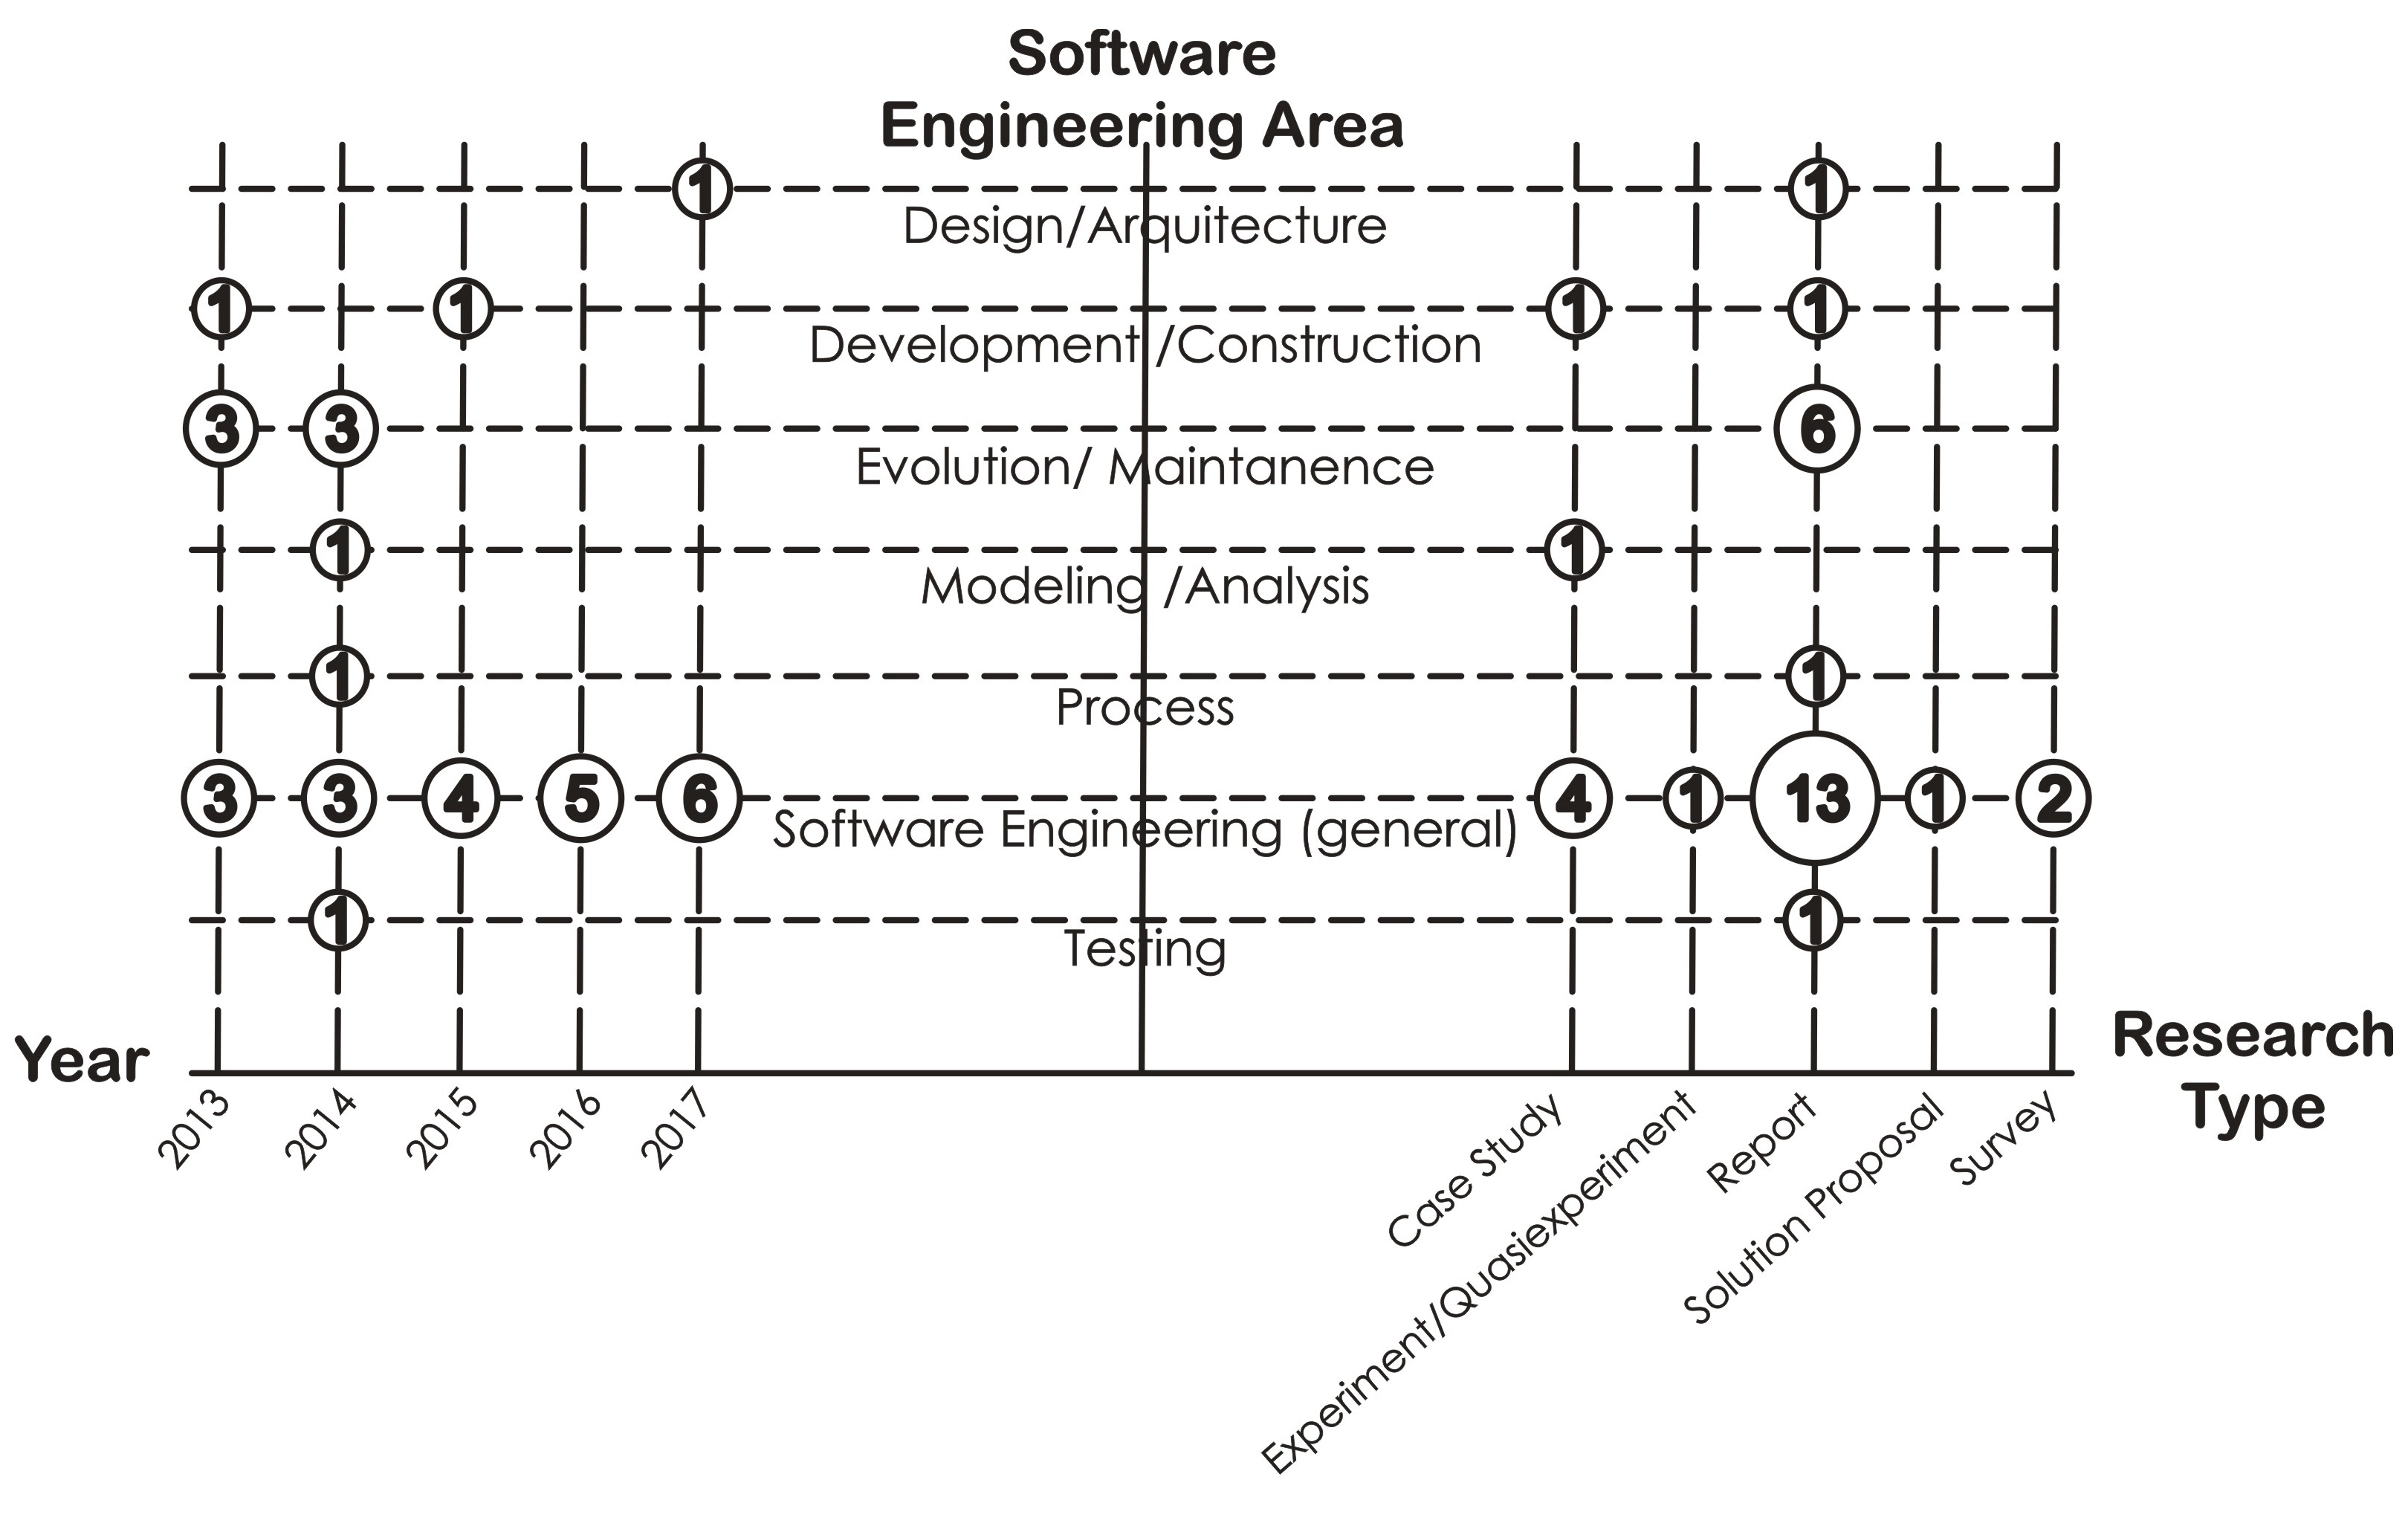
\includegraphics[width=0.8\linewidth]{fig/mapa01.jpg} 
\caption{Software engineering area vs. year vs. research type.} \label{fig:mapa01}
\end{figure*}

\subsection{Overview of study objectives and contributions}

We have identified several approaches in the selected papers. One of the main challenges of using FLOSS in SE education is selecting projects for use in a course. Some studies address the choice of suitable projects, providing a predefined list of FLOSS \cite{id0135, id5357, id5676}. \citeauthor{id0135} made available a list of seventeen projects compatible with students' background. The selected projects ranged in size from 5,500 to 10,500 lines of code. \citeauthor{id5357} have listed ten open source projects for exploring, experimenting and choice by students. In the study of \citeauthor{id5676}, students choose the project from a list presented in the classroom. 
%
In some studies, students freely choose the project they wanted to work during the course 
\cite{id1088, id17882}. 
In the study presented by \citeauthor{id1088}, teams were able to freely choose a project to carry out their practices and apply the software development techniques learned in lectures. 
\citeauthor{id17882} let students choose a software system to study its architecture and to document the system. 
In the study of \citeauthor{id0093}, authors specify a set of criteria to aid the selection process. Groups of up to six students undertook a search for projects hosted in the SourceForge, GitHub and GoogleCode repositories. \citeauthor{id1192} previously established that students should work with the JabRef project, an open source bibliographic reference manager.

Some studies present techniques for using FLOSS in SEE \cite{id0106, id0134, id1192, id17800, id5676}. \citeauthor{id0106} used the Wilcoxon Mann-Whitney test, a non-parametric statistical hypothesis test, to compare two related samples. The result of their tests led to reject the null hypothesis that confirmed the efficacy of the method. 
In their study, \citeauthor{id0134} subjected students 
to the technique of visualizing algorithms, showing parameters, relevant variables, 
and visual representation of manipulated objects, as well as a formal description of the algorithm. Students reported that software visualization tools are easy to use and help understand software structure, behavior, and complexity. 
\citeauthor{id1192} used gamification to guide and motivate students to contribute to FLOSS projects. \citeauthor{id17800} provided a tutorial to help instructors identify appropriate software projects, design the set of tasks for students, and select useful tools. \citeauthor{id5676} used a hybrid approach combining distance-based project learning, providing printed materials (e.g., books, tutorials and articles), online resources and classroom lectures.

We identified tools that served to support the use of open source projects in SEE \cite{id1088, id17882, id5357, id0089, id5676}. \citeauthor{id1088} and \citeauthor{id17882} used the Github version control system to maintain project code and track individual student contributions. In the study of \citeauthor{id5357}, student pairs were able to develop, test, and debug small Java programs using Eclipse and to create UML class diagrams. The study of \citeauthor{id0089} reports the experience of an open source software community using the GitLab teaching environment to support students' collaborative software development activities. \citeauthor{id5676} gave their students access to the FLOSSCom and OpenSE virtual learning environments.

Other studies have described their assessment processes \cite{id4663, id0093, id0089, id5676}. 
For \citeauthor{id4663}, project grade accounts for 70\% of students' scores. They considered product usefulness, maintenance capacity, extension of software design, verification effectiveness, teamwork and final presentation. In~\cite{id0093}, students were assessed from code presentation, participation in communication channels, documentation submitted at each stage, comments from peer review and contribution to the FLOSS community repository. To assess students, \citeauthor{id0089} considered push, pull, and commit records that students performed using GitLab. Finally, in \cite{id5676} the assessment considered the quality of produced work, documentation clarity and usefulness, number of bugs reported, complexity and effectiveness of developed code, and analysis depth and usefulness.

% Mapa02 aqui - burlando latex
\begin{figure*}[htb]
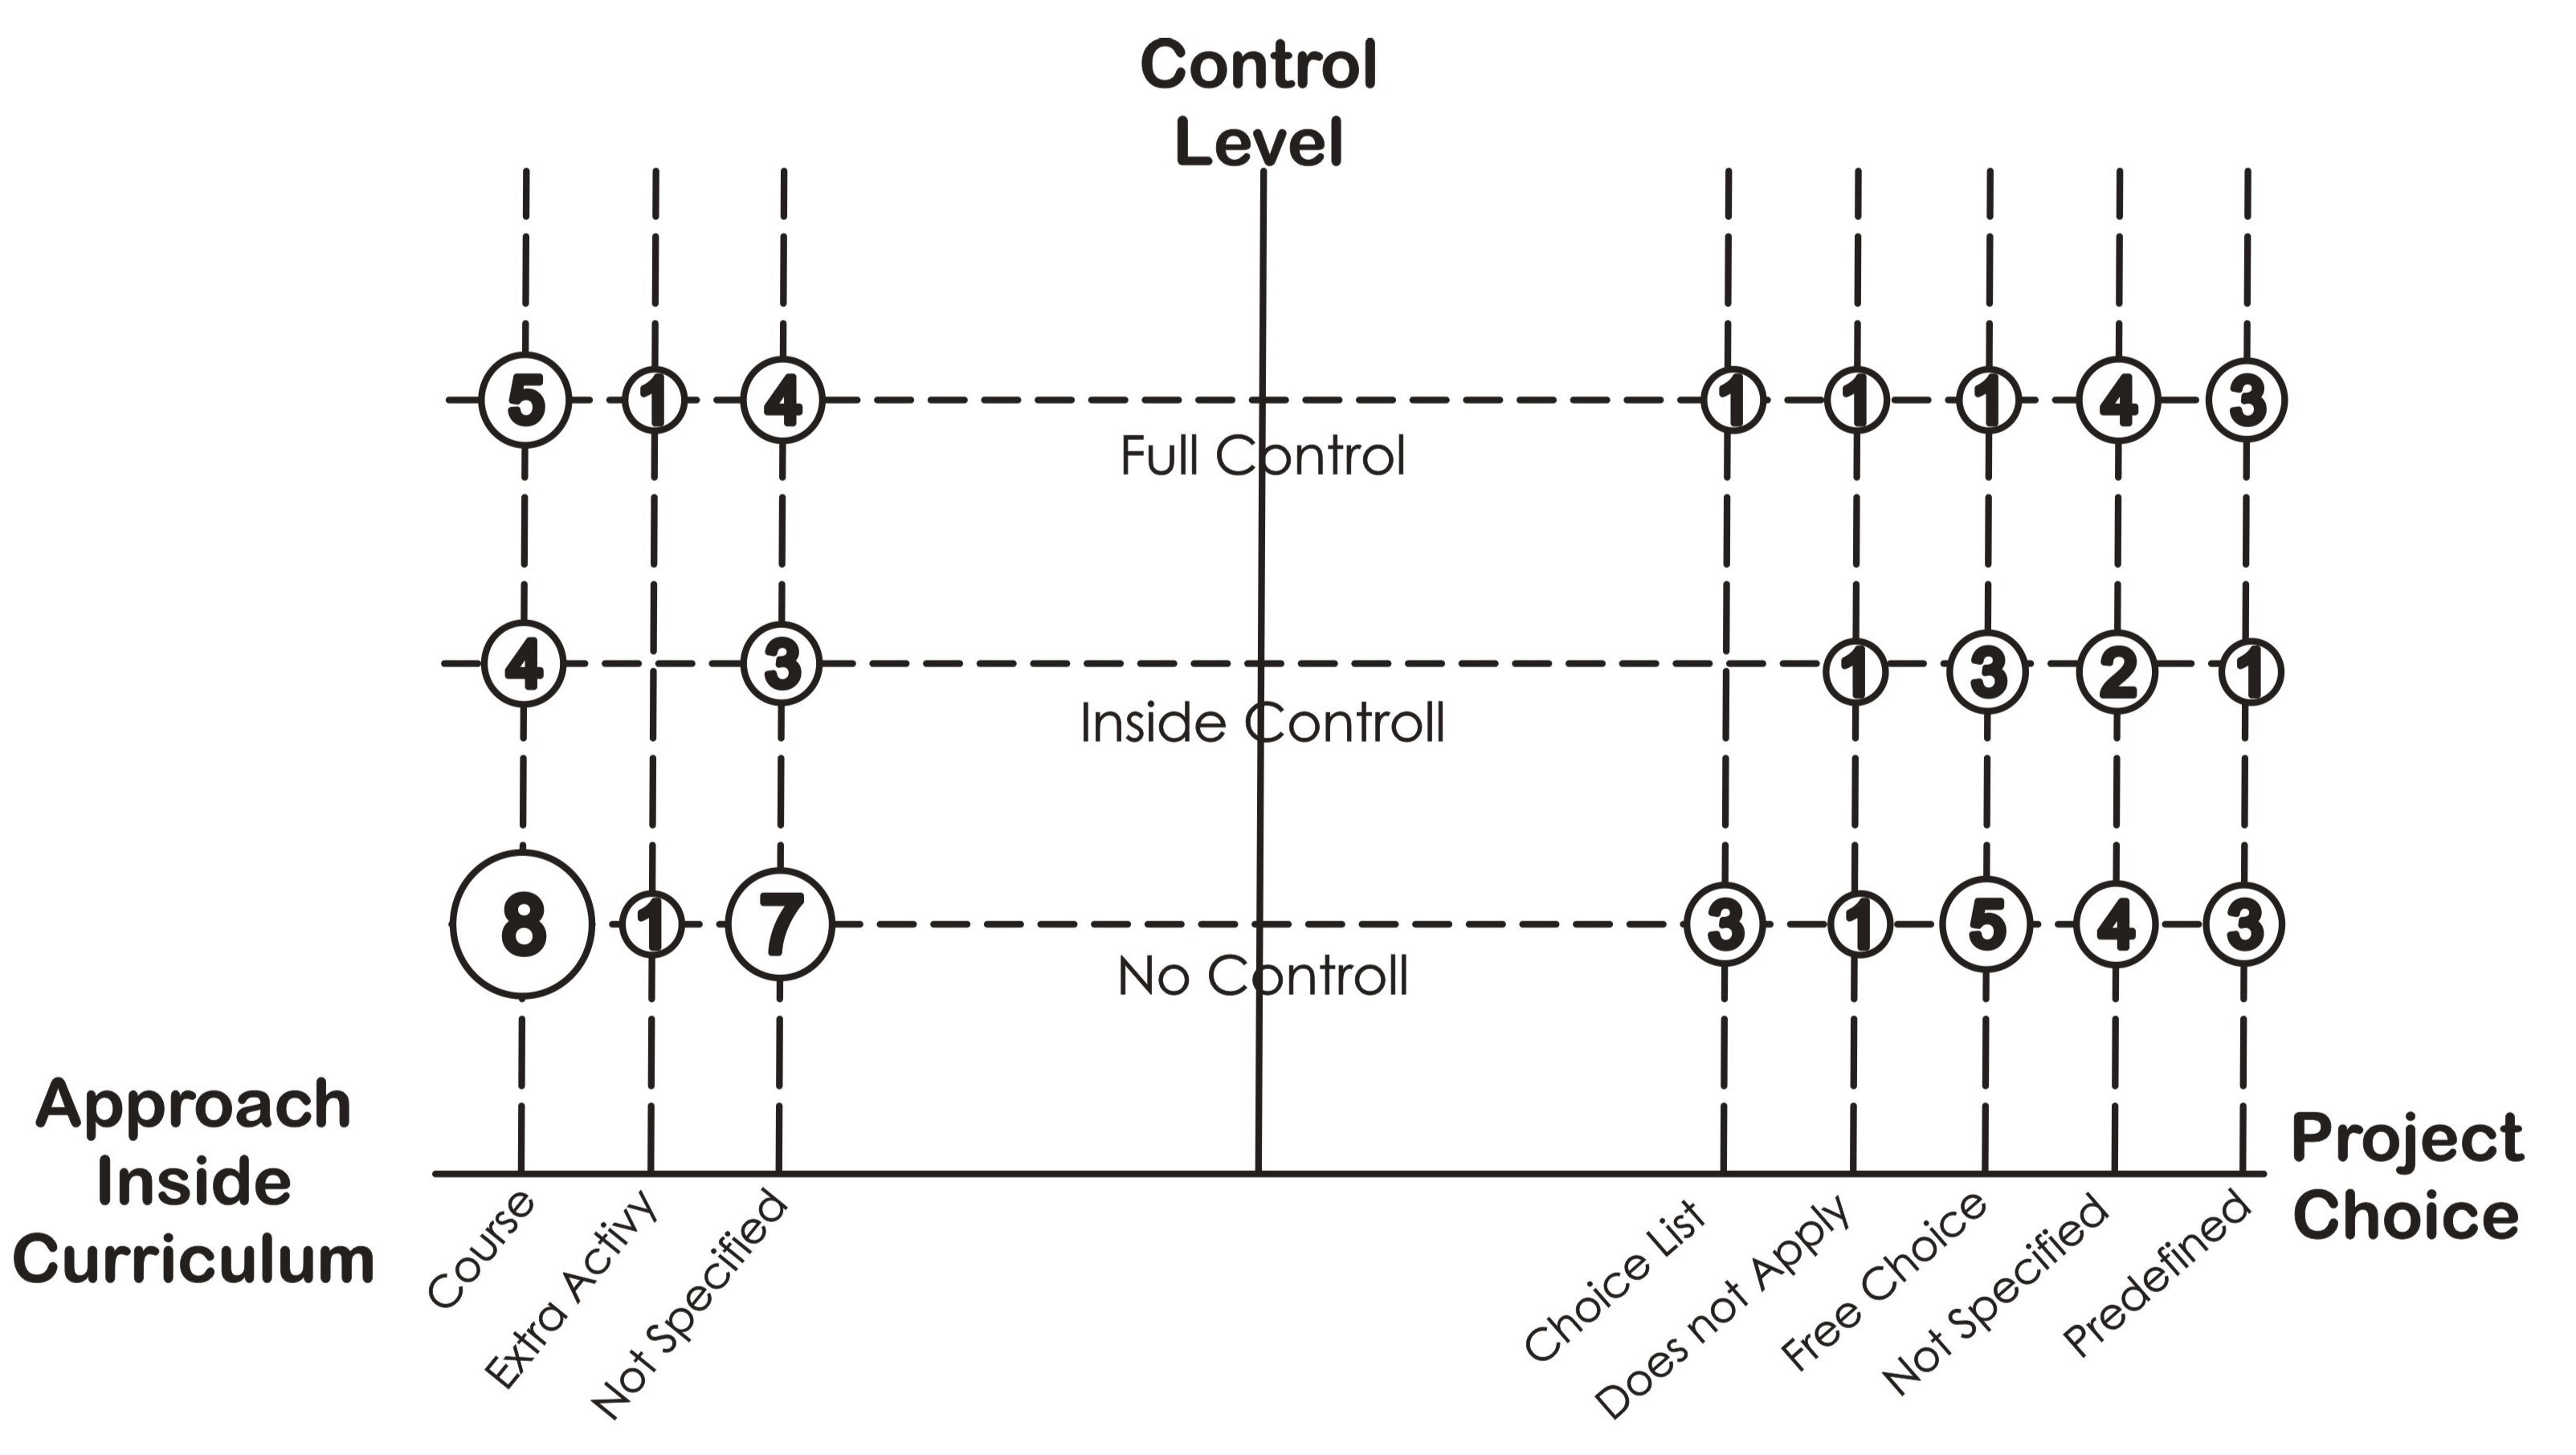
\includegraphics[width=0.7\linewidth]{fig/mapa02.jpg}
\caption{Curriculum choice vs. control level vs. project choice.} \label{fig:mapa03}
\end{figure*}

\subsection{FLOSS projects in SEE}

The main purpose of our SMS update was to discover 
how FLOSS projects have been used in SEE (RQ1) 
over the last five years. 
Figure~\ref{fig:mapa01} presents a map 
that combines Facet~1 - Software Engineering Area, 
Facet~2 - Research Type and year of publication.

%We perform an analysis on each facet. 
%Starting with 
% tab-seArea-Studies

%\begin{table*}
\begin{table}[bt]
	\centering
	\caption{Studies classified by \it Facet 1 - Software Engineering Area}
		{\begin{tabular}{l|p{1.3in}|r }
			\bf Area & \bf Studies & \bf \# \\
			\hline
			Software Engineering & \citep{id0093, id1088, id4503, id4663, id4811, id4815, id5676, id17805, id17830, id17845, id18433, id5329, id5335, id0098, id0106, id1097, id1192, id1193, id4966, id5147, id18359} & 21 \\
			Evolution/Maintenance & \citep{id0135, id5343, id5353, id17796, id0115, id17800} & 6 \\
			Development/Construction &  \citep{id0089, id5546} & 2 \\
			Design/Architecture & \citep{id17882} & 1 \\
			Modeling/Analysis & \citep{id0134} & 1 \\
			Process & \citep{id5357} & 1 \\
			Testing & \citep{id5328}  & 1 \\		
		\end{tabular}} \label{tab:seAreaStudies}
\end{table}
%\end{table*}


\paragraph{Facet 1 - Software Engineering Area}
Table~\ref{tab:seAreaStudies} shows how primary studies addressed software engineering areas.
Twenty-one studies (63.6\%) deal with the general software engineering area. There was a small decrease of 5.8\%, 
when compared to the results from the previous SMS~\cite{2015:CSE:nascimento}. 
Twelve studies (36.3\%)  were focused on particular software engineering areas. 
Evolution/Maintenance leads the count with six papers, followed by Development/Construction with two papers and 
Design/Architecture, Modeling/Analysis, Process and Testing,
with only one study each.
No papers were found that relate FLOSS projects with the knowledge areas of
Requirements, Quality, Management and Configuration Management.

% tab-researchType-Studies

\begin{table}[bt]
	\centering
	\caption{Studies classified by \it Facet 2 – Research Type}
		{\begin{tabular}{l|p{1.6in}|r}
			\bf Category & \bf Studies & \bf \# \\
			\hline
			Experience report & \citep{id17882, id0135, id5343, id5353, id17796, id5357, id1088, id4503, id4663, id4811, id17805, id17830,id17845,id18433, id5329, id5335, id0089, id0115, id17800, id0106, id4966, id18359, id5328} & 23 \\
			Case study & \citep{id0093, id4815, id5546, id0134, id1192, id1193} & 6 \\
			Experiment &  \citep{id5676} & 1 \\
			Survey/questionnaire & \citep{id0098, id5147} & 2 \\
			Proposal of solution & \citep{id1097} & 1 \\	
		\end{tabular}} \label{tab:researchTypeStudies}
\end{table}


\paragraph{Facet~2 - Research Type}
Table~\ref{tab:researchTypeStudies} presents the research methods used in primary studies.
Twenty-three papers fall into the experience report category, representing 69\% of the selected papers. 
There was an increase in this type of study, given that, in the previous mapping~\cite{2015:CSE:nascimento}, 
this category represented only 19.4\% of the studies analyzed. 
The category named solution proposal, the most popular
in~\cite{2015:CSE:nascimento}, was found only once in our update. 
This work reports that empowering students to become socially responsible professionals is a desirable outcome of SEE, 
and humanitarian free and open source software (HFOSS) projects provide an opportunity for educators to inspire students to face global humanitarian challenges (realistic settings) while learning about software engineering \cite{id1097}. 
While no Experiment/Quasi-Experiment had been found in the previous SMS, 
this update found one work \cite{id5676} in this category. 
\citeauthor{id5676} reported the results after four years performing an instructional method that uses FLOSS projects as tools to teach a software engineering course.

\subsection{Fitting FLOSS projects into students’ activities}

Figure~\ref{fig:mapa03} presents a map that combines 
Facet~8 - Control Level, Facet~7 - Curriculum Choice 
and Facet~9 - Project Choice to show
how FLOSS projects have been integrated into students' activities over the last five years. 

% tab-approachCurriculum-Studies

\begin{table}[htb]
	\centering
	\caption{Studies classified by \it Facet 7 - Curriculum Choice}
		{\begin{tabular}{l|p{2.0in}|r }
			\bf Category & \bf Studies & \bf \# \\
			\hline
			Extra activity & \citep{id5329, id5335} & 2 \\
			Course & \citep{id17882, id0135, id5343, id5353, id17796, id5357, id0093, id1088, id4503, id4663, id4811, id4815, id5676, id17805, id17830, id17845, id18433} & 17 \\
			Not specified & \citep{id0089, id5546, id0115, id17800, id0134, id0098, id0106, id1097, id1192, id1193, id4966, id5147, id18359, id5328} & 14 \\
		\end{tabular}} 	\label{tab:approachCurriculumStudies}
\end{table}


Table~\ref{tab:approachCurriculumStudies} shows the results 
for Facet~7 - Curriculum Choice. 
Most studies still incorporate FLOSS projects into regular course curriculum (17 articles). In a different approach, two studies used FLOSS in extra activities, while 14 articles did not specify how they used it.

Two papers presented experiences in elective courses \citep{id0093, id5353}. \citeauthor{id0093} present the experience of preparing students to take on the roles and responsibilities of an incoming software engineer. 
\citeauthor{id5353} report a preliminary study on the combination 
of research and education in software testing. 

Four articles describe experiences with undergraduate students \citep{id0089, id0106, id4663, id5328}. 
\citeauthor{id4815} explore the participation of master's students 
in FLOSS projects, mixing the learning contexts of formal and open/informal education. 
\citeauthor{id0134} and \citeauthor{id1097} report experiences in teaching and learning programming. 
Finally, two primary studies
present approaches based on extra activities \cite{id5329, id5335}. 
\citeauthor{id5329} describe two courses taught at two universities, built around a model of communities of practice, and present lessons learned. 
\citeauthor{id5335} report an approach where students are 
involved in an HFOSS project shared with the GNOME Accessibility 
team and four academic institutions.

Table~\ref{tab:controlLevelStudies} presents the results for Facet~8 - Control Level. 
We classified the studies according to 
three different categories on how much 
the faculty / staff controlled student activities.
The majority of the studies, corresponding to 48.4\% (16 papers),
used approaches where instructors had no control over the activities carried out by students. 
This scenario differs from the previous SMS, where there was a balance between approaches where instructors had either inside control or no control over student activities. 

The no control approach emphasizes the real-world experience, 
as students will need to interact with the project community, users and developers. As an example of this approach,  \citeauthor{id4815} used mailing list, chats, and forums to exchange ideas and doubts or to share achievements by using the channels used by the FLOSS community. Moreover, the final part of the project requires a work submission to relevant communities of each project. In another example, \citeauthor{id5546} aimed to identify what should be learned about software development through active participation in FLOSS communities. In both examples, instructors only monitor students activities. 

This SMS update identified only seven papers (21.2\%) that fit into inside control category, 
where there is no required interaction with the community, and usually the instructor uses a project as an independent branch. 
\citeauthor{id0106} describe the process of cloning an open source module 
and how students use structured modeling, such as data flow diagrams, 
functional decomposition, and UML diagrams, to reverse engineer the cloned module.
Finally, we found ten studies characterized as 
full control, where the core of the FLOSS community are 
the faculty themselves. 
Compared to the original mapping, 
we had an increase from 12.5\% to 30.3\% of studies that adopted this category. 
This might indicate the growing interest of academia for developing their own projects. 
It might also mean that is is easier to choose a project known by their academic staff. 
\citeauthor{id0134} provide an example of this approach: 
they picked out an open source project, some student-developed programs, 
and two software visualization tools, and then applied them 
in a programming course for students to evaluate the use of software visualization 
in teaching and learning programming.

% tab-controlLevel-Studies

\begin{table}
	\centering
   
	\caption {Studies classified by \it Facet 8 - Control Level}
		\begin{tabular}{l|p{2.0in}|r}
			\bf Category & \bf Studies & \bf \#  \\
			\hline
			No control & \citep{id5343, id5357, id4663, id4815, id5676, id17805, id17830, id17845, id5335, id5546, id0098, id1192, id1193, id4966, id5147, id5328} & 16 \\ 
			Inside control & \citep{id17882, id17796, id0093, id18433, id0089, id0106, id1097} & 7 \\
			Full control & \citep{id0135, id5353, id1088, id4503, id4811, id5329, id0115, id17800, id0134, id18359} & 10 \\ 
		\end{tabular} \label{tab:controlLevelStudies}
\end{table}


Table~\ref{tab:projectChoiceStudies} presents the results
for Facet~9 - Project choice, and it
gives us insights into how selected studies deal with project selection appropriate for FLOSS adoption in computing courses.
We identified that students worked in free-choice projects on most papers where authors specified the way projects were selected, 
diverging from the previous mapping which claimed that, 
in general, students worked in predefined projects. 

Eight papers whose project selection was free choice, such as \citeauthor{id17882} and \citeauthor{id5343}, allowed students to choose any real-world open source project for use in the SE course. We noted that \citeauthor{id17796} and \citeauthor{id0098} gave students the freedom to choose the projects. 
However, this choice process was supervised by the instructor so that the chosen projects should meet certain conditions/constraints, e.g.,  project size, active design and number of developers. The study presented by \citeauthor{id5357} looked at students' motives for choosing open source projects for use in a maintenance-focused software engineering course. 

In seven studies, students worked on predefined projects. For instance, \citeauthor{id5329} chose the Ubuntu project for all their students to work with, since such a project has several options for contributors, including documentation, design, development, bugs and tests. \citeauthor{id1192} chose JabRef, a consolidated FLOSS project, where one of the authors is part of the project maintenance team, which facilitated instrumenting it. 

Finally, we found five studies where instructors provided a list of projects for students. Among those studies, we may cite \citeauthor{id0135}, that manually searched and evaluated about 1000 projects from various FLOSS projects repositories and chose 17 projects that were compatible with their students' previous experiences. 
As in the previous mapping, we also identified studies that provided a list of FLOSS projects options, but students were free to choose a project that was not in the list \cite{id5546}.

% tab-projectChoice-Studies

\begin{table}
	\centering
	\caption {Studies classified by \it Facet 9 - Project Choice}
		{\begin{tabular}{l|p{2.0in}|r}
			\bf Category & \bf Studies & \bf \#  \\
			\hline
			Predefined & \citep{id5353, id4503, id18433, id5329, id5335, id1192, id5147} & 7 \\
			Choice list & \citep{id0135, id1088, id4815, id5676, id17830} & 5 \\
			Free choice & \citep{id17882, id5343, id17796, id5357, id0093, id17845, id5546, id0098} & 8 \\
			Not specified & \citep{id4663, id0089, id0115, id17800, id0134, id0106, id1193, id4966, id18359, id5328} & 10 \\
			Does not apply & \citep{id4811, id17805, id1097} & 3 \\
		\end{tabular}}
	\label{tab:projectChoiceStudies}
\end{table}


Unlike the previous SMS, 
Figure 3 shows that studies with full control level are not always predefined for students. 
We identified studies with full control where project choice was either from a list \cite{id0135} or chose by free choice \cite{id1088}. 
We identified 69.7\% of the studies (23 articles) with either no control or inside control. As in the previous mapping, most studies without a level of control, students had free choice over their projects. 
Regarding the combination of Facet~7 - Curriculum Choice and 
Facet~8 - Control Level, we realized that most studies in regular courses have no control. 
In the previous SMS scenario, 
most studies with internal control were somewhat more common in regular courses.

\subsection{Assessing students}

Table~\ref{tab:approachGoalStudies} presents the results
for Facet~6 - Approach goal. 
In this facet, concepts were developed and discussed in a systematic way. 
We observed that, in the last 5 years, 
16 studies were classified in the 
``Learning about FLOSS projects in a Software Engineering Course'' 
category, and 17 studies in the 
``Learning about SE concepts using FLOSS projects'' category. 
Thus, there was a balance between 
the approach goals, differentiating our mapping from the previous one. 
Consequently, we perceived an interest of the academic community in 
how students have learned about FLOSS projects.
This interest has been confirmed by \citeauthor{id1088}, 
who asserted that introducing SE students to FLOSS projects 
exposes them to challenges such as 
those that they will face as professional software developers.

% tab-approachGoal-Studies

\begin{table}[h]
	\centering
	\caption {Studies classified by \it Facet 6 - Approach Goal}
		{\begin{tabular}{l|p{2.1in}|r}
			\bf Category & \bf Studies & \bf \# \\
			\hline
			Learning SE & \citep{id17882, id0135, id5343, id5353, id5357, id4503, id4811, id4815, id5676, id17805, id17845, id5546, id17800, id0134, id0106, id5147, id5328} & 17 \\
			Learning OSS & \citep{id17796, id0093, id1088, id4663, id17830, id18433, id5329, id5335, id0089, id0115, id0098, id1097, id1192, id1193, id4966, id18359} & 16 \\
		\end{tabular}} 
        \label{tab:approachGoalStudies}
\end{table}



Table~\ref{tab:assessmentTypeStudies} describes
the studies of Facet~5 - Assessment Type. 
Software artifacts (7 studies) and Reports (7 studies) 
are still the main assessment instruments used by instructors 
in studies where learning was explicitly assessed.
However, from five primary studies,
we identified a new category, which we named ``Passing Tests'', 
that was not mentioned in the previous SMS.

% tab-assessmentType-Studies

\begin{table}[htb]
	\centering
	\caption{Studies classified by \it Facet 5 - Assessment Type }
		{\begin{tabular}{l|l|r}
			\bf Category  & \bf Studies  & \bf \#  \\
			\hline
			Exams & \citep{id5546} & 1 \\
			Reports & \citep{id17882, id5343, id4815, id5676, id17805, id17845, id5335} & 7 \\
			Software artifacts & \citep{id5353, id0093, id1088, id4503, id4663, id5329, id0089}  & 7 \\
			Passing Tests & \citep{id0135, id0115, id0134, id0106, id1192} & 5 \\
			Portfolio & \citep{id4811} & 1 \\
			None & \citep{id17796,id5357, id17830, id18433, id17800, id0098, id1097, id1193, id4966, id5147,id18359, id5328} & 12 \\
		\end{tabular}}
	\label{tab:assessmentTypeStudies}
\end{table}


% Burlando latex
\begin{figure}[t]
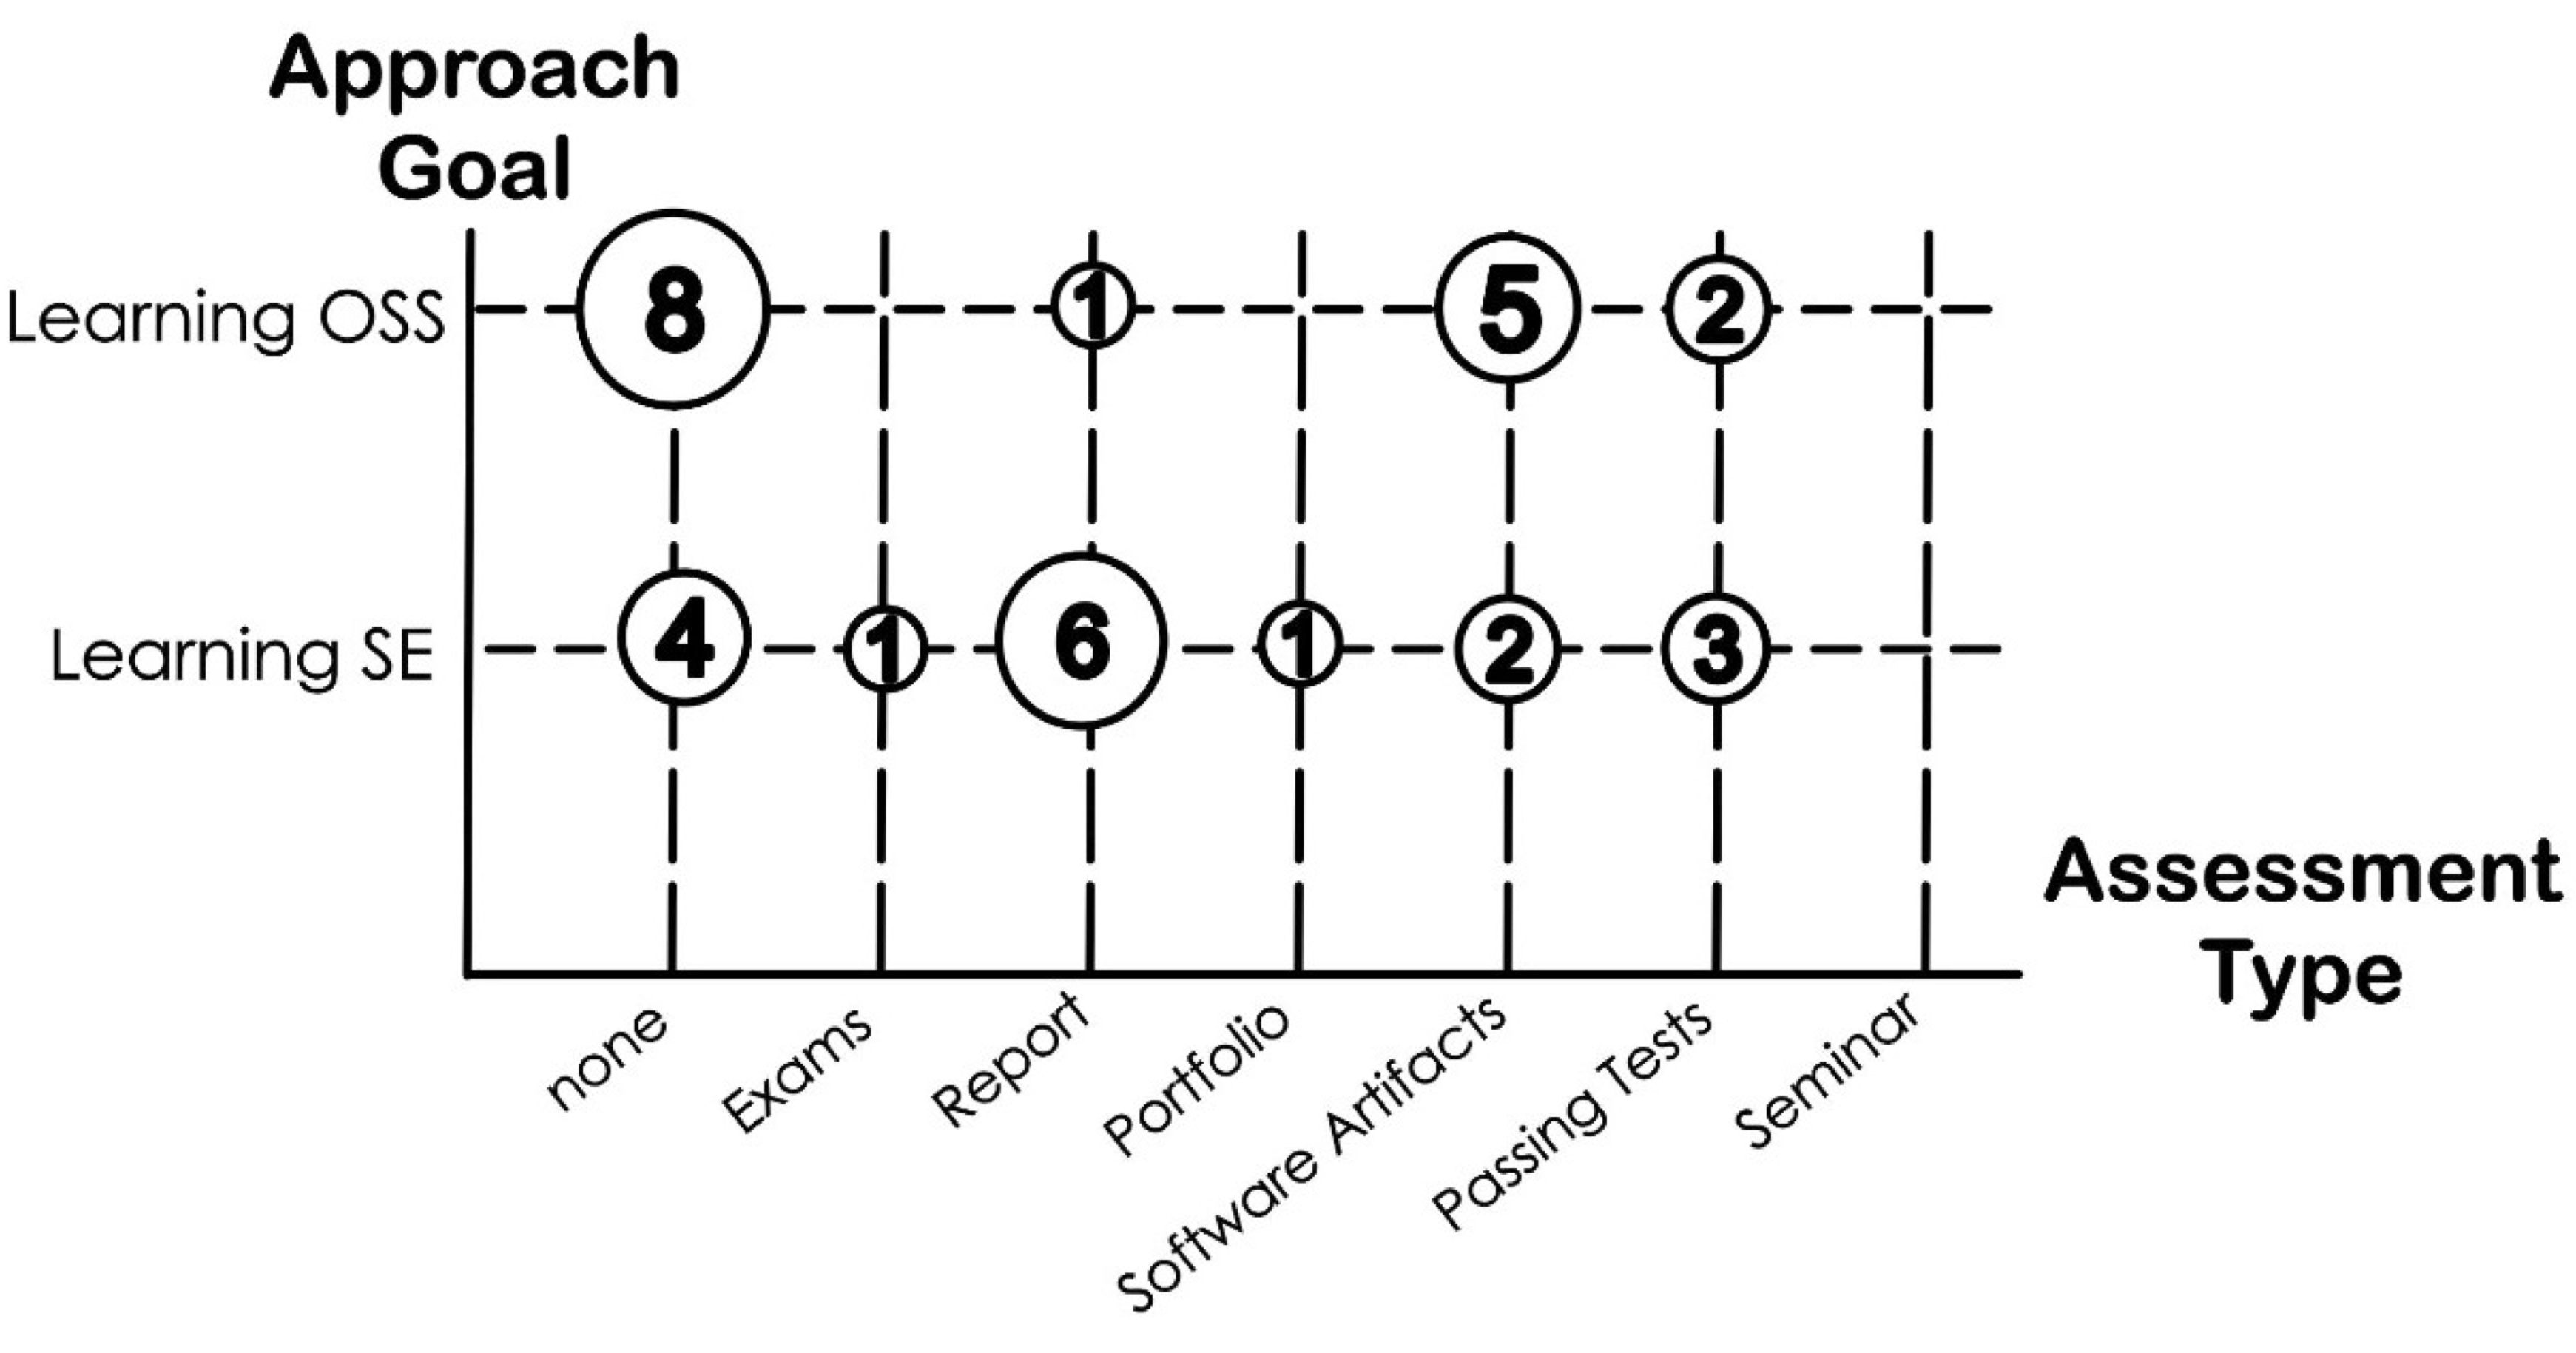
\includegraphics[width=\linewidth]{fig/mapa03.jpg}
\caption{Approach goal vs. assessment type.} \label{fig:mapa04}
\end{figure}

The map in Figure ~\ref{fig:mapa04} presents
an overview of how assessment occurs in the selected studies.
This map combines Facet 6 - Approach Goal with the Facet 5 - Assessment Type.
The primary studies are listed in Tables ~\ref{tab:approachGoalStudies} and ~\ref{tab:assessmentTypeStudies}.
% ESCLARECER: We identified the student assessment perspective from the general goals of the studies (Table ~\ref{tab:assessmentTypeStudies}).

Most studies with the general goal of teaching SE concepts and principles 
used reports (6 articles), 
passing tests (3 articles) and software artifacts (2 articles). 
The study described by \citeauthor{id4811} used exams, and the study of \citeauthor{id4811} used a portfolio. 
In studies with the goal of teaching OSS, predominantly no assessment was explicitly performed. 
From these studies, five papers used software artifacts and two other papers used passing tests. 
Only in the study of \citeauthor{id5335}, reports were used as assessment, 
although it was the predominant assessment type in the studies 
aiming to teach SE concepts and principles.

\subsection{Distribution of publications}

In the last five years, the interest of the research community
on the use of FLOSS projects in SEE has evolved. 
We present a temporal view of publications, main publication venues and the institutions that devote more effort to this subject.

\subsubsection{Temporal view}

\begin{figure}[ht]
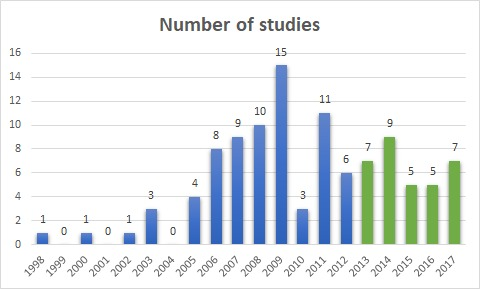
\includegraphics[width=\linewidth]{fig/number_of_studies.jpeg}
\caption{Publications vs. year.} \label{fig:publicationsvsyear}
\end{figure}

Figure~\ref{fig:publicationsvsyear} shows the distribution of publications over the years. 
The green bars refer to the number of studies identified 
in this present mapping. 
There has been a growing interest in this subject over the years. We notice an almost constant interest after a 2009 peak and a sharp fall in 2010. There is a balance in the number of studies that were published in the last five years, with a small increase in 2017 compared to 2016.

\subsubsection{Publication venues}

\begin{table}
\caption{Main Publication Venues}
{\begin{tabular}{p{3.05in}|c}
\textbf{Venue} & \textbf{\#} \\ \hline
FIE - Frontiers in Education Conference  & 3 \\
ICCSE - Intern. Conference on Computer Science \& Education & 3 \\
SIGCSE - ACM Technical Symposium on Computer Science Education & 2 \\
CSEE\&T - Conference on Software Engineering Education and Training & 2 \\
ASEE Annual Conference and Exposition & 2 \\
Journal of Computing Sciences in Colleges & 2
\end{tabular}} 
\label{tab:publicationVenue}
\end{table}


Table~\ref{tab:publicationVenue} presents the distribution of articles by venue, considering venues that published two or more selected papers. The complete set of publication venues (each with only article from the 33 selected articles) 
can  be found in our mapping study website\footnote{https://moara.github.io/mapping/}.  Most studies are still published in important conferences, 
such as the Frontiers in Education Conference (FIE) and the ACM Technical Symposium on Computer Science Education (SIGCSE). 
In the previous mapping, the Annual Conference on Innovation and Technology in Computer Science Education (ITiCSE) was identified as the second largest publication venue. In this mapping, however, only one paper was published in this conference.
The International Conference on Computer Science \& Education (ICCSE), not
identified in the previous mapping, shows up with three papers included in this update.

Figure~\ref{fig:temporalViewpublicationsources} shows how this topic has been addressed in the last five years. As in the previous systematic mapping, conferences remain the typical place to publish results (19 papers). Journals are the second most popular venue (9 papers). There was only one paper published in 2017 in both workshops and as books or book chapters. Finally, symposiums were also popular for publishing results, both in 2014 (3 paper) and in 2017 (1 paper).

\begin{figure}[ht]
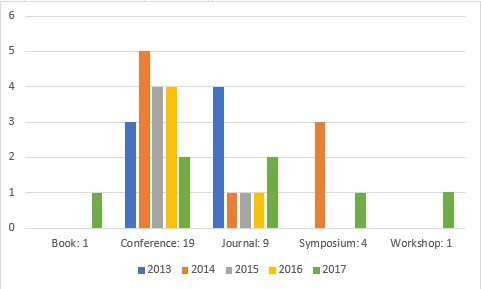
\includegraphics[width=\linewidth]{fig/types_of_venue.jpeg}
\caption{Temporal view and publication venues.} \label{fig:temporalViewpublicationsources}
\end{figure}

\subsubsection{Active research communities}

To learn which institutions have devoted effort to studying student participation in FLOSS projects as an approach to learn SE, we looked at affiliation details in our selected studies.
Table~\ref{tab:communities} summarizes the communities that had at least two selected  publications in this mapping study. 

\begin{table}[htb]
\caption{Active Research Communities}
{\begin{tabular}{p{3in}|c}
\textbf{Institutions} & \textbf{\#} \\ \hline
Drexel University, US & 7 \\
Western New England University, US & 7 \\
University of Connecticut, US & 4 \\
Nassau Community College, US & 3\\
Western Oregon University,  US & 3\\
Northern Arizona University, US & 2\\
California State University, Chico, US & 2\\
University of Minho, Portugal & 2\\
The College of New Jersey, US & 2\\
Muhlenberg College, US & 2\\
Moravian College, US & 2
\end{tabular}}
\label{tab:communities}
\end{table}



% Posicionei manualmente
\begin{figure*}[ht]
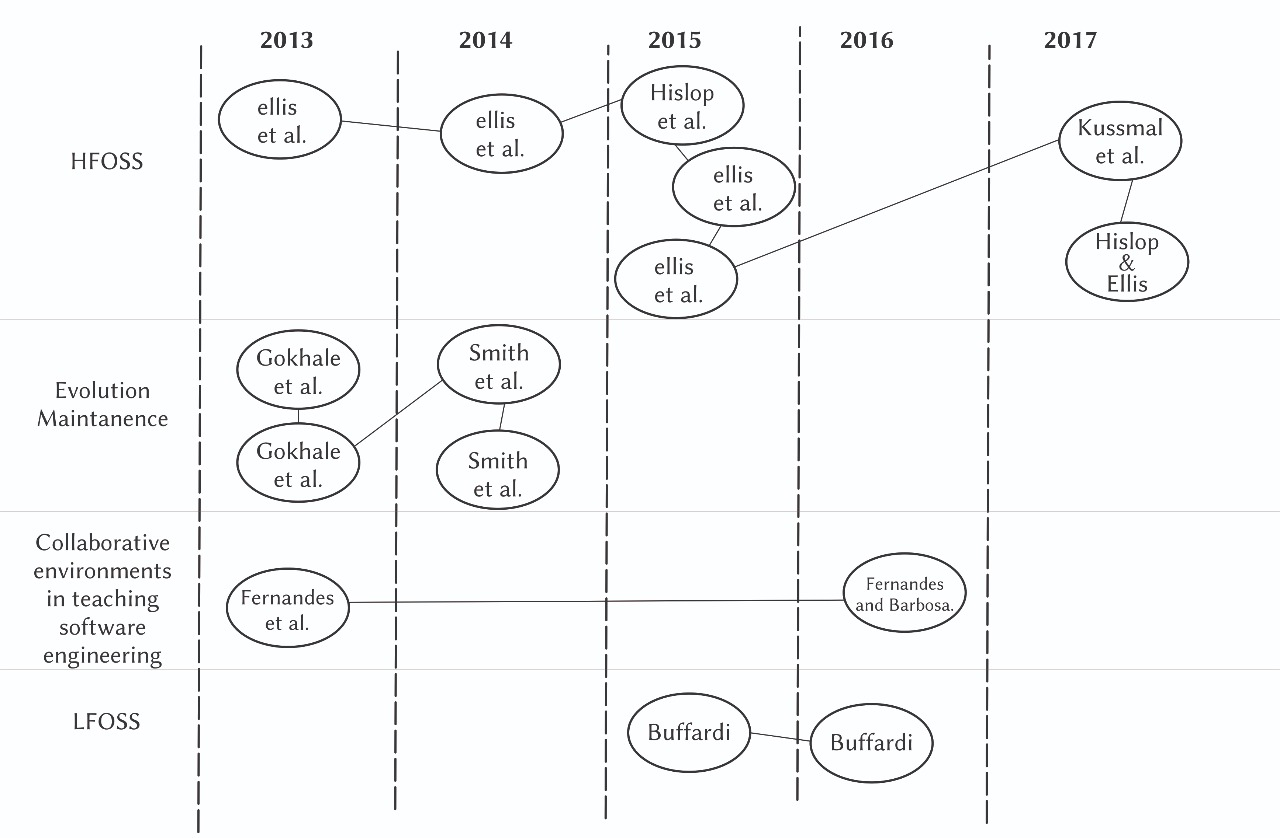
\includegraphics[width=.8\linewidth]{fig/long_term.jpeg}
\caption{Long-term projects.} \label{fig:longterms}
\end{figure*}

Communities such as Drexel University and Western New England University, 
which are related to the Humanitarian Free and Open Source Software project (HFOSS), continue to produce the largest number of studies. These communities reeived contributions from other communities that were not identified in the previous mapping. 
They are: 
Nassau Community College, Muhlenberg College, The College of New Jersey, Western Oregon University, Moravian College. 
Among the communities cited in \citeauthor{2015:CSE:nascimento} as contributors to HFOSS, only Bowdoin College was identified in our mapping. 
Drexel University and Western New England University keep very relevant 
to the research community, not only because of the number of published studies, 
but also because of their involvement with a number of other communities. 
We have not identified Trinity College community-related publication within the past five years, although they have published 12 studies in the previous mapping. 
Regarding the Aristotle University of Thessaloniki and North Carolina State University, 
who respectively published four and three papers in the previous mapping, 
we found only one study in each of them.
The University of Connecticut published two papers in 2012 
(which were previously identified), 
and four papers between 2013 and 2014. 
After that, we did not find other publications from this community 
about the use of FLOSS in SEE.

Two new communities appeared in the current mapping: 
University of Minho, which published two studies related to collaborative environments in teaching software engineering (FLOSS approach), and Northern Arizona University, which attracted attention by having two Brazilian authors 
(an Associate Professor at the Northern Arizona University (NAU) and member of the Computer Science Graduate Program at the University of São Paulo, and a Post-Doctoral Scholar at the School of Informatics, Computing and Cyber-Systems at NAU, and Assistant Professor at the Federal University of Technology - Paraná). 
They conducted research related to supporting newcomers in open source software development communities, including student involvement in FLOSS projects.

\subsection{Long-term projects}

As we read the articles included in the mapping, we tried to capture the  maturity of each solution proposal in each study, based on how long or how many times it had been applied. 
The scenario is similar to the previous mapping, with studies strongly related to others, and with few cases, since most of the identified studies continue to apply the proposed solution only once. Figure~\ref{fig:longterms} presents studies whose solution proposals were applied twice or more, and each linked set of nodes represents one identified project. 

The largest identified project was HFOSS, with seven studies.  \citeauthor{id1193} describes a workshop held to prepare faculty members to deliver courses in which students participate in HFOSS software development projects. The 2014 study \cite{id5335} and one 2015 study \cite{id4966} describe student learning within the environment of an HFOSS project. The other two 2015 studies (\cite{id5147, id17830})
report students' opinions about the learning and impact of their participation in an HFOSS project. After one year without particular publications on the use of open source projects in SEE, in 2017 we identified two publications with general information on Humanitarian Open Source Software in Computing Education \cite{id1097,id18359} and information to faculty and students on how to participate in the Humanitarian Free and Open Source software OpenFE and OpenPath.

The University of Connecticut has developed a long-term project. The first studies published in 2013 \cite{id17800,id0135} describe experiences and lessons learned from using FLOSS to teach software maintenance and evolution. 
The following papers, published in 2014 \cite{id17796,id5357},
refer to the search, by instructors and students, of projects suitable for use in SEE with a focus on maintenance and evolution.

The study of \citeauthor{id4815} is based on a pilot project in teaching and learning software engineering that has been carried out for two years. 
The first findings were reported by \citeauthor{id5546} in 2013.

In 2015, \citeauthor{id1088} described the Localized Free and Open Source Software organization - LFOSS (an
experimental approach to combine advantages of collaborating
with industry with maintaining existing open source projects), and reports initial findings from software engineering students' involvement. In this study, he also describes the Chico Open Source Consortium (COSC) as a group in Chico, California, to foster collaboration between California State University-Chico (CSU Chico) students and local software professionals in open source projects. In the following year, a new report of a more realistic software development experience was published, continuing to focus on LFOSS \cite{id4663}.


%\section{Trends} \label{sec:trends}
%\section{Discussion} \label{sec:discussion}

To the best of our knowledge, this is the first research work that investigates
the sustainability of academic software regarding its publicization, evolution
stage in the life cycle, and recognition. 
We performed three exploratory studies in the domain of
academic software for static analysis, based on software publications from ASE
and SCAM, two relevant software engineering conferences. ASE is more general in
scope and SCAM is concerned with source code analysis.

\paragraph{\bf Evolution of the recognition of academic software for static
analysis published in ASE and SCAM} The academic software has received more
attention in the academic literature over time; there is a clear
growth in the total number of references to software for static analysis in
publications of the ACM and IEEE databases, as Figure~\ref{mentions-by-year}
shows.

\begin{figure}[ht]
  \centering
  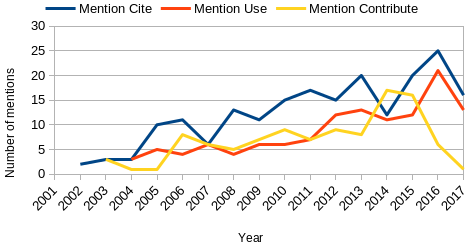
\includegraphics[scale=0.59]{figs/mentions-type-by-year.png}
  \caption{Total number of mentions per type and year.}
  \label{mentions-by-year}
\end{figure}

This growth, however, may be influenced by the increase in the number of
projects each year. By isolating the data and keeping the number of projects
constant over time, there is a growth of 38\% per year, according to
Figure~\ref{mentions-trend}.

\begin{figure}[ht]
  \center
  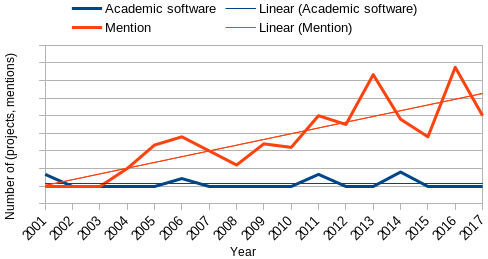
\includegraphics[scale=0.59]{figs/mentions-trend.png}
  \caption{Growth in the number of mentions per year.}
  \label{mentions-trend}
\end{figure}

Among the 60 academic software projects of static analysis studied, 13 projects
(22\%) did not have academic recognition, i.e., they were mentioned only in
the original article published in ASE or SCAM, where the software was introduced. The
other 47 projects (78\%) had greater academic recognition, whereas mentions
have been found in one or more articles other than the first publication.

\paragraph{\bf Influence of the life cycle stage on the recognition of academic
software} There were 160 mentions for projects in close-down stage.
This data
possibly indicates that papers published before the project enter this stage or
indicating that the project is accessible only to its authors but not for the
general public.
%
For other life cycle stages, we found 71 mentions for projects
in evolution or servicing stages and 131 mentions for projects in the initial
development stage.

We found a large number of mentions for ESBMC, PARSEWeb,
and TestEra, including recent publications
between 2016 and 2017; however, the fact that they are in the close-down stage
demands attention, since they are not publicly available but continue to
receive attention from academia.


\section{Conclusion} \label{sec:conclusion}
% Conclusion

We presented an update to a systematic mapping study
performed by our research group in 2013 to investigate
the use of FLOSS projects in Software Engineering Education. 
%
The first mapping selected 72 primary studies,
published from 1998 to 2012, and
categorized them according to nine facets 
(software engineering area, research type, learning approach,
assessment perspective, assessment type, 
approach goal, curriculum choice, control level and project choice).
The updated mapping selected 33 primary studies
published from  2013 to 2017, and
categorized them according to the same nine facets.
%
Moreover, we compared the results to provide
a comprehensive overview on how FLOSS projects have been used in the context of SEE in the last 20 years.

There has been a steady but yet small body of research 
that addresses the pedagogical use of FLOSS projects in SEE; 
it includes 105 primary studies, developed by a small number of
groups and researchers, and mostly published in conferences 
on computer science education.
% with a growing number of publications and researchers interested in the subject.
From 105 studies in 20 years, 
only one was classified as Experiment/Quasi-experiment in
the Research Type facet.
Despite the increase in the number of experience reports,
evidence shows that the research area is not mature yet.

%
The updated SMS is a valuable asset both 
to researchers interested in the identified trends and gaps, and 
to instructors interested in trying out their own experiences in their classes. 





\bibliographystyle{ACM-Reference-Format}
\bibliography{bib/sbes2018-et-bibliography}

\appendix
\section{Facets} \label{sec:facets}

% Assessment Type
\begin{table}[hbt]
\centering
\caption {Assessment Type - Facet 5}
   \vspace{-0.25cm}
   \begin{small}
   {\begin{tabular}{l|p{2.25in}}
		\bf Category & \bf Description \\ \hline
			\bf Exams & Students are assessed by means of written exams. \\
			\bf Reports & Students should write a report for assessment. \\
		    \bf Software artifact & Students assessed through developed artifacts. \\
%			\bf Passing Tests & Automated tests such as unit tests are used to assess performed work. \\
			\bf Interviews & Interviews are conducted to assess learning. \\
			\bf Seminars & Students assessed by performance in seminars. \\
%			\bf Portfolio & Students should produce a portfolio as result of their work. \\
			\bf Exercises & Students assessed by means of exercises. \\
			\bf Surveys & A survey is conducted to assess learning. \\
			\bf Reflective essay & A reflective essay is written. \\
			\bf Presentations & Students assessed by presenting their work. \\
			\bf Participation & Student's participation in class, in community, interaction with group or team. \\
			\bf None & No assessment instrument mentioned in paper. \\
			\bf Does not apply & Not related to activity where assessment is needed. \\

		\end{tabular}} \label{tab:assessmentType}
        \end{small}
\end{table}


% Curriculum Choice
\begin{table}[h]
	\centering
	\caption {Curriculum Choice - Facet 7}
        \begin{small}
            \vspace{-0.25cm}
		{\begin{tabular}{l|p{2.2in}}
			\bf Category & \bf Description \\
			\hline
			\bf Extra activity & Students worked with FLOSS in extra activities, e.g., internships. \\
			\bf Capstone Project & Students worked with FLOSS in a capstone project. \\
			\bf Course & Working with FLOSS was a student's assignment in a regular course. \\
			\bf Not specified & The paper does not mention where, in the curriculum, the approach is used. \\
			\bf Does not apply & Related to an experience where curriculum issues are not declared. \\
		\end{tabular}} \label{tab:curriculumApproach}
        \end{small}
\end{table}


% Control Level
\begin{table}[h]
	\centering
	\caption {Control Level - Facet 8}
   \vspace{-0.25cm}
        \begin{small}
		{\begin{tabular}{p{0.9in}|p{2.2in}}
			\bf Category & \bf Description \\
			\hline
			\bf No control & Faculty/staff only monitor student's activities inside the project. Students work with community requests and the community approves students' contribution.  \\ % Everything that is necessary for the project is defined and approved by its community.
			\bf Inside initiative/ External approval & A new feature is proposed and built inside college, but later, it is submitted to community approval.\\
			\bf Inside control & Faculty/staff branch the FLOSS code, prepare assignments, and evaluate themselves the students' contribution. \\
			\bf Full control & Project core development has been sustained by faculty/staff. \\ % The core team of the OSP is the faculty staff. The project is generated and maintained inside the college
			\bf Not specified & No control level could be identified in the paper. \\
			\bf Does not apply & Work is not related to an experience where control level is needed. \\
		\end{tabular}} \label{tab:controlLevel}
   \end{small}
\end{table}


% Project Choice
\begin{table}[hb]
	\centering
	\caption {Project Choice - Facet 9}
    \begin{small}
		{\begin{tabular}{l|p{2.2in}}
			\bf Category & \bf Description  \\
			\hline
			\bf Predefined & Faculty/staff decide the project students work. \\
			\bf Choice list & Students can choose any project from the list provided by faculty/staff. \\
			\bf Free choice & Students should seek and decide which OSP (from their interest) they will work with. \\
			\bf Not specified & Paper does not mention issues related to project choice. \\
			\bf Does not apply & Work is not related to an experience where choosing a project is needed. \\
		\end{tabular}} \label{tab:projectChoice}
    \end{small}
\end{table}


\end{document}
